%-------------------------------------------------------------------------------------------------------------------------VPN
\section{Virtual Private Networks}
Una rete privata virtuale consiste in una rete il cui accesso è regolamentato, che si appoggia a un protocollo di trasporto pubblico e condiviso, e che consente di garantire confidenzialità della comunicazione, accesso solo previa autenticazione, integrità dei dati e protezione da alcuni tipi di attacchi, ad esempio Man-in-the-middle o attacco replay.

\subsection{Architetture disponibili}
Una rete VPN può realizzare diversi tipi di collegamenti, per soddisfare esigenze diverse. Nei paragrafi successivi, si andranno ad analizzare i 3 tipi di architetture più comuni:
\begin{itemize}
    \item \textbf{Gateway-to-Gateway}: consiste in una VPN che connette in maniera stabile due reti. Questa configurazione permette ad esempio di estendere una rete privata tra diverse location geograficamente separati e distanti a piacere, oppure di garantire a una serie di uffici un accesso sicuro a un data center;
    \item \textbf{Host-to-Host}: questa configurazione è la meno comune. Consiste nello stabilire una comunicazione diretta tra due host, in cui uno fa da server VPN e l'altro da client VPN. Un caso d'uso potrebbe essere un amministratore di sistema che deve fare gestione remota di un apparecchio;
    \item \textbf{Host-to-Gateway}: in questa modalità, il risultato che si ottiene è lo stesso che si avrebbe connettendo un host alla rete locale in cui risiede il server VPN. È usata principalmente per offrire un accesso sicuro da remoto alla rete. Quando l'host vuole instaurare una connessione VPN con il server, gli viene richiesto di autenticarsi.
\end{itemize}

Una VPN in configurazione Host-to-Gateway si prospetta come la soluzione più pratica e funzionale per soddisfare le necessità dell'azienda e dei suoi dipendenti, garantendo loro la possibilità di accedere alle risorse interne attraverso un canale di comunicazione privato, ad accesso controllato, criptato e dove è assicurata l'integrità dei dati.

\begin{figure}[ht]
    \centering
    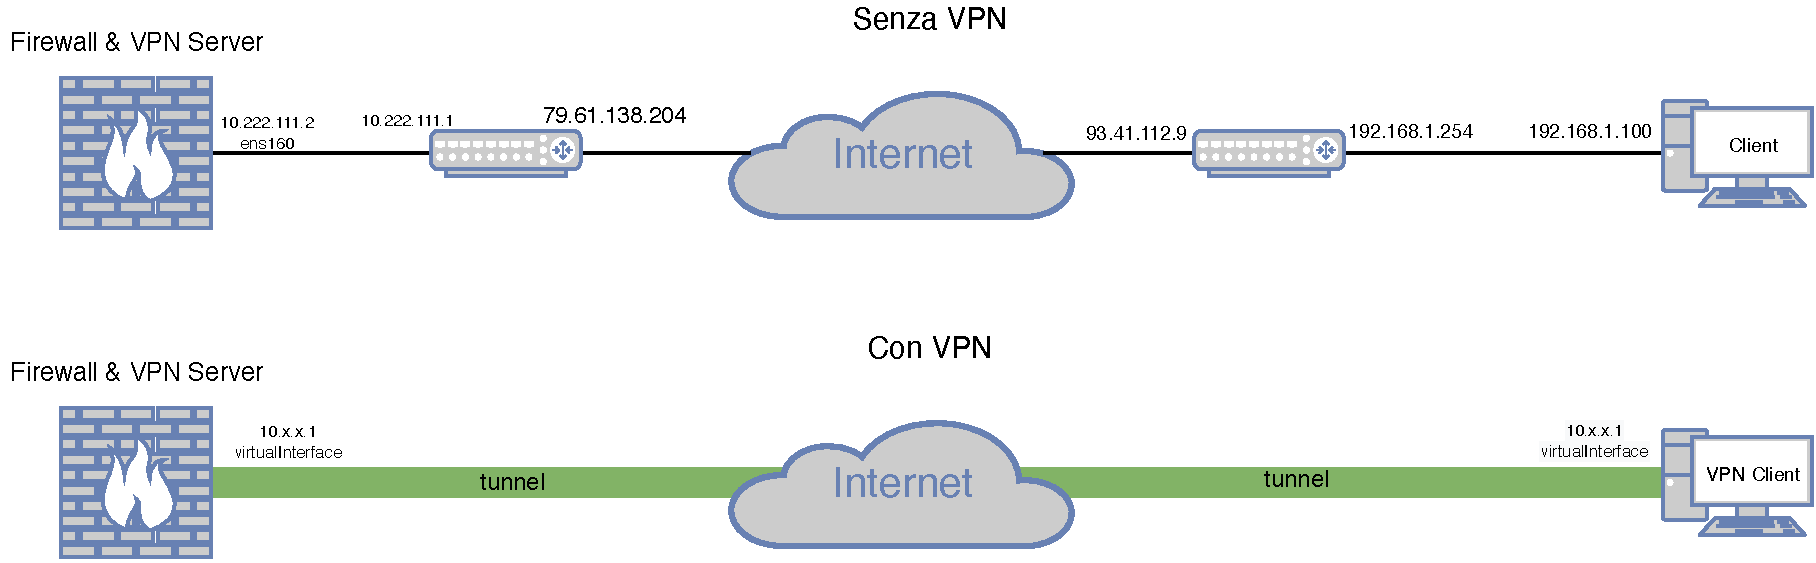
\includegraphics[width=10cm]{figure/vpn_noVPN.pdf}
    \caption{Modello logico di connessione con e senza VPN}
\end{figure}

\section{Soluzioni VPN più comuni}

Tra le soluzioni VPN più comuni troviamo:
\begin{itemize}
    \item Point-to-Point Tunneling Protocol (PPTP);
    \item Internet Protocol Security (IPSec);
    \item OpenVPN;
    \item WireGuard.
\end{itemize}

%-----------------------------------------------------------------------------------------------------------------------IPSec
% BUONO https://pctempo.com/openvpn-vs-ikev2-vs-pptp-vs-l2tp-ipsec-vs-sstp/

% https://it.wikipedia.org/wiki/IPsec https://github.com/sunknudsen/privacy-guides/blob/master/how-to-self-host-hardened-strongswan-ikev2-ipsec-vpn-server-for-ios-and-macos/README.md 

% 1.	Come è nato
% 2.	Tipo incapsulamento
% 3.	Overhead - byte sprecati per pacchetto
% 4.	Livello a cui lavora
% 5.	Protocolli usati
% 6.	Cifratura usata ? hw o sw, limitata se non aggiorni hw ma più veloce, e il contrario

\subsection{Internet Protocol Security}
\subsubsection{Panoramica}
IP Security è una suite di protocolli il cui obiettivo è rendere sicura la comunicazione tra due computer attraverso una rete IP.
Contiene protocolli per la mutua autenticazione degli host e per la negoziazione delle chiavi di cifratura da usare durante la sessione.
In molti contesti, rendere sicuro il livello di rete (L3 OSI) è una soluzione migliore rispetto a rendere sicuro il livello di trasporto (L4 OSI) o di presentazione (L7 OSI), in quanto offre un ulteriore punto di controllo per gli amministratori e più flessibilità nell'analizzare, e gestire, ogni singolo pacchetto IP.
IPSec supporta l'autenticazione a livello di rete, autenticazione del mittente, integrità dei dati, cifratura, e protezione dagli attacchi replay, protezione dall'analisi del traffico e controllo degli accessi.

\subsubsection{Transport mode vs Tunnel mode}
La suite IPSec può essere configurata per lavorare o in transport mode o in tunnel mode.
\begin{figure}[ht]
    \centering
    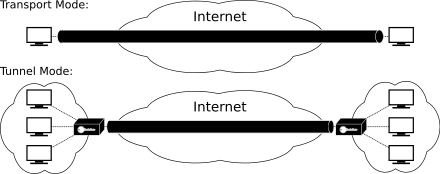
\includegraphics[width=8cm]{figure/ipsec_modes.png}
    \caption{Transport mode vs Tunnel mode diagram}
\end{figure}


\noindent \textbf{Transport mode}

In transport mode, generalmente solo il payload del pacchetto IP è cifrato o autenticato. L'indirizzamento non cambia, dato che l'header IP non è né modificato né cifrato; tuttavia, quanto si usa il protocollo Authentication Header, approfondito in seguito, l'indirizzo IP non può essere modificato da Network Address Translation (NAT), in quanto una modifica al campo invaliderebbe l'hash. Il livello di trasporto e di applicazione sono sempre certificati da un hash, quindi il loro contenuto non può essere modificato in alcun modo, ad esempio utilizzando una traduzione dei numeri delle porte.
Un superamento delle problematiche causate dall'attraversamento di NAT è definito dalle RFC che descrivono il meccanismo NAT-T, ma che va oltre gli scopi di questa tesi.

\newpage
\noindent \textbf{Tunnel mode}

In tunnel mode, l'intero pacchetto è cifrato e autenticato. È dunque incapsulato all'interno di un nuovo pacchetto IP con un nuovo header IP.
Generando un nuovo header IP, non si incontra nessuna difficoltà nell'attraversamento di NAT.


\subsubsection{Protocolli utilizzati}
IPSec utilizza i seguenti protocolli per stabilire una connessione sicura. Sia AH che ESP, descritti in seguito, possono lavorare in tunnel mode o in transport mode.

\noindent \textbf{Authentication Header}

\begin{figure}[ht]
    \centering
    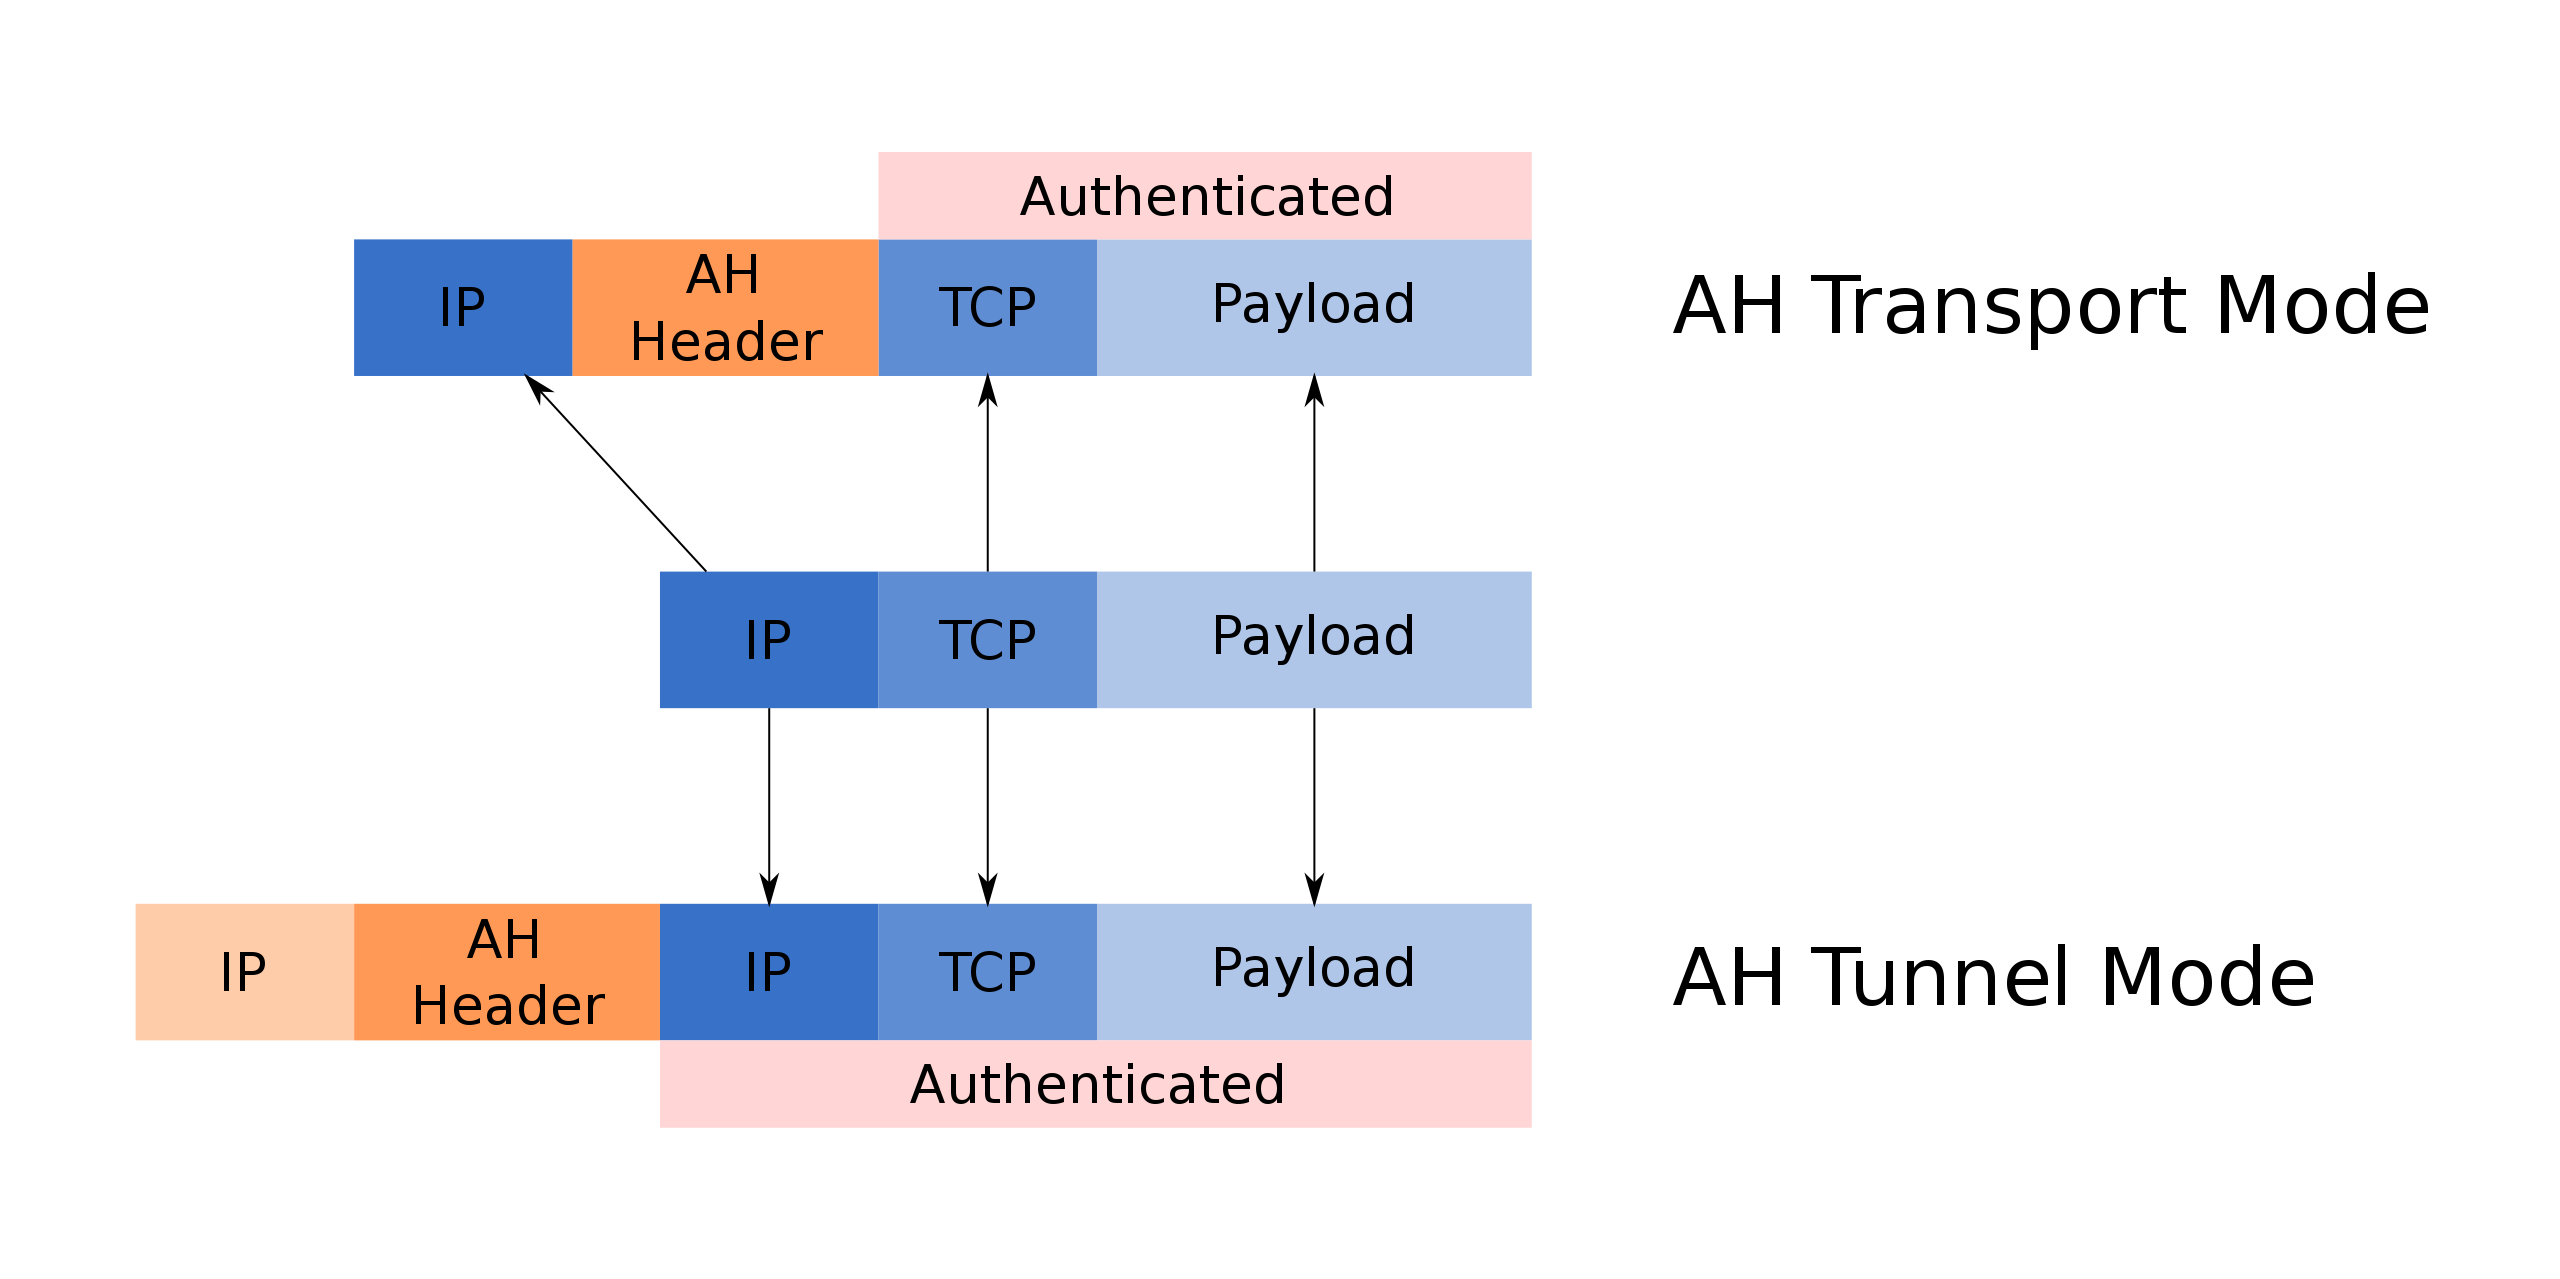
\includegraphics[width=10cm]{figure/ah_tun_trasp.png}
    \caption{Formato del pacchetto di Authentication Header}
\end{figure}

Authentication Header \cite[RFC4302]{RFC4302} (AH) garantisce integrità per tutti gli header dei pacchetti, ad eccezione di alcuni campi dell'header IP, e autenticazione del mittente. Se configurato, è anche possibile utilizzarlo per offrire protezione dagli attacchi replay. AH si interfaccia direttamente con IP, utilizzando il protocollo IP numero 51.
AH autentica l'intero datagramma, ad eccezione dei campi variabili. Tuttavia, le informazioni contenute nel datagramma sono trasferite in chiaro e, dunque, leggibili da uno sniffer. Per questo motivo, AH non soddisfa i requisiti di sicurezza richiesti.

\noindent \textbf{Encapsulating Security Payload}

\begin{figure}[ht]
    \centering
    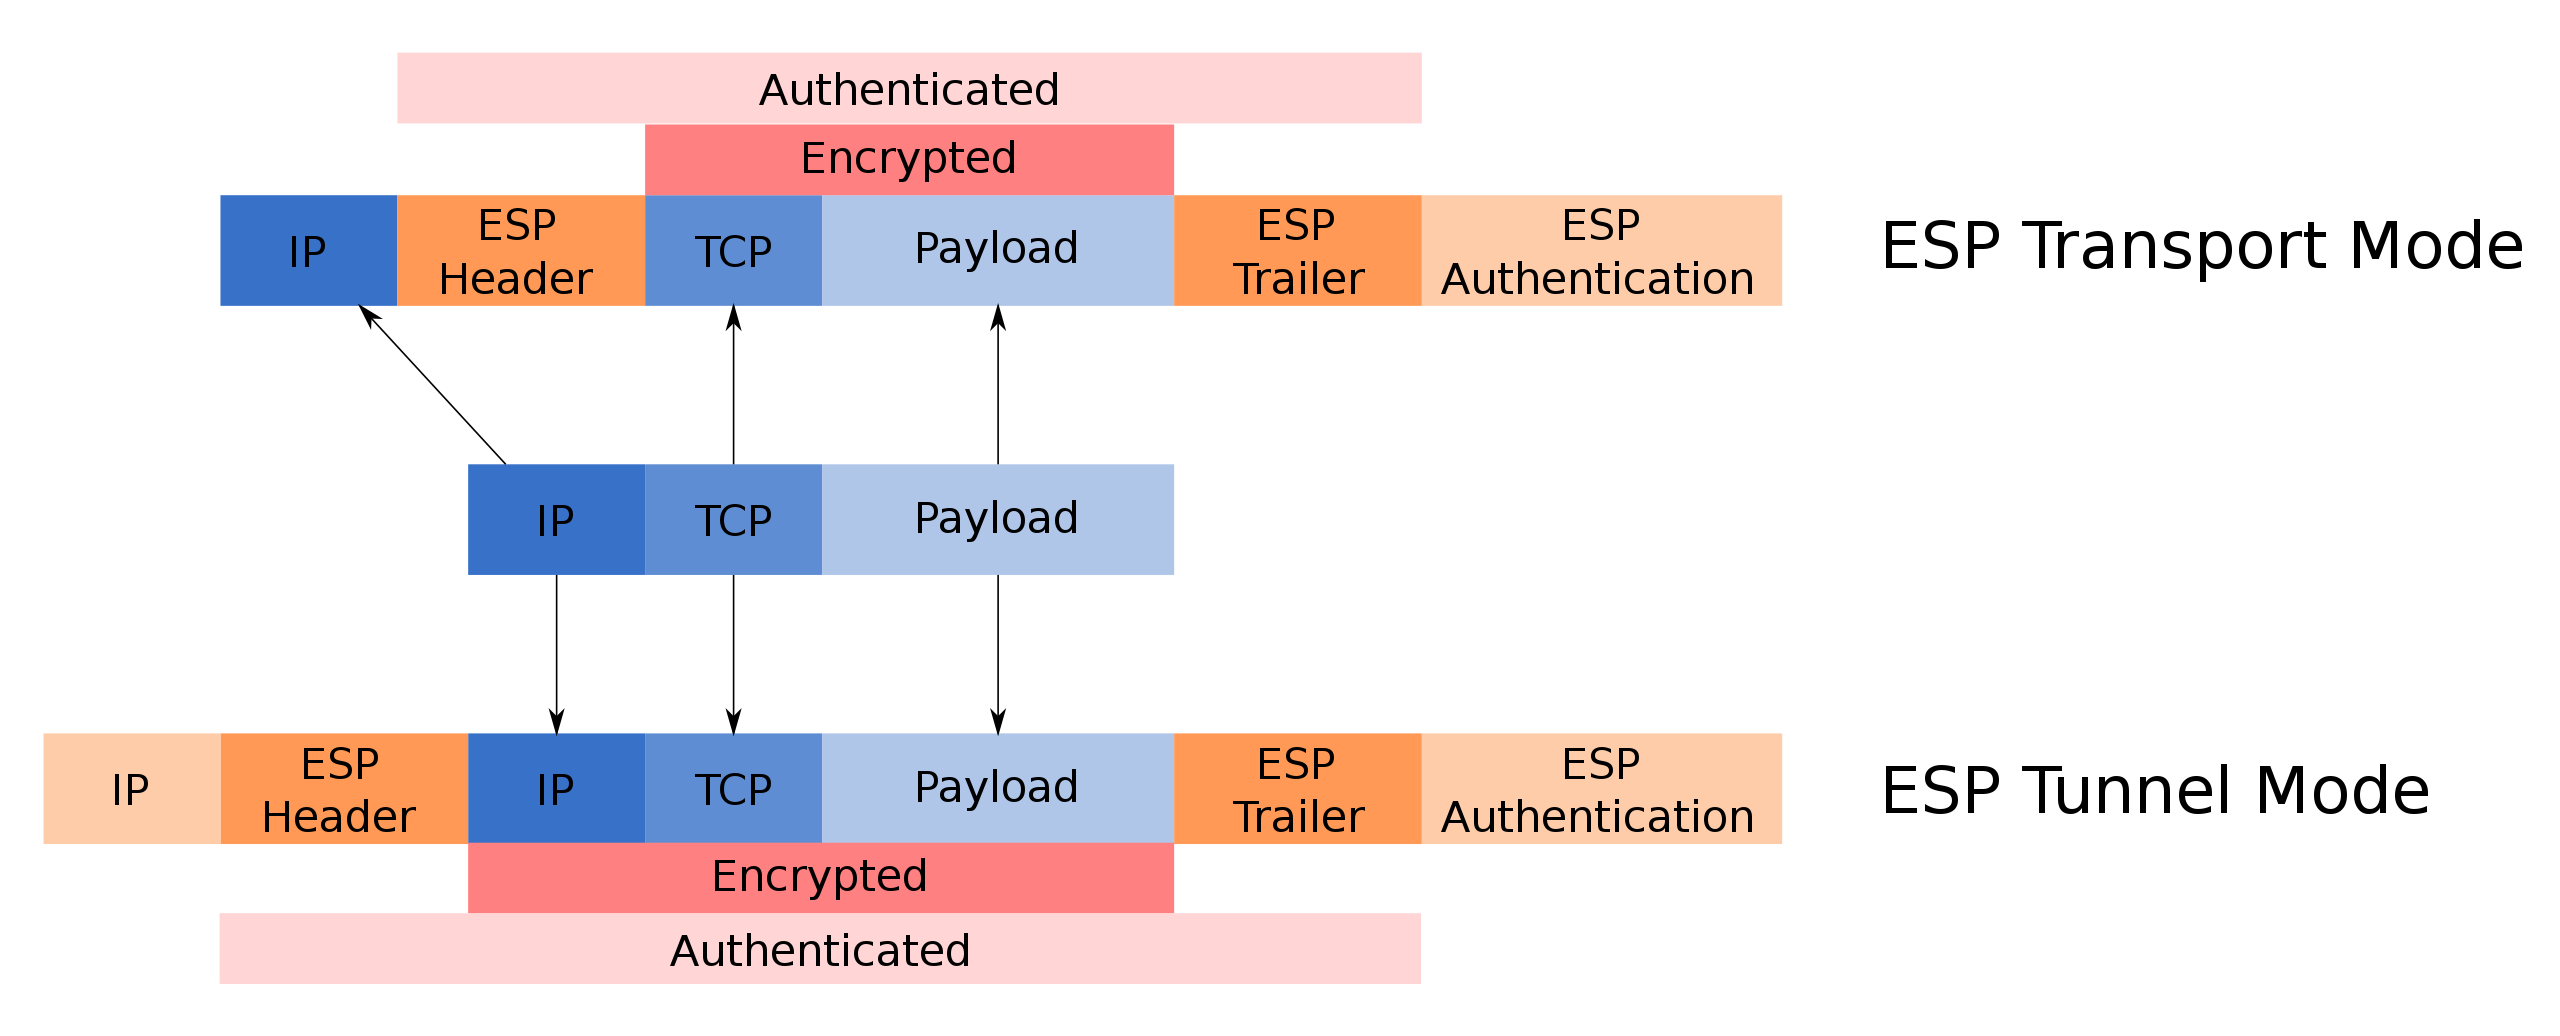
\includegraphics[width=10cm]{figure/esp_tun_trasp.png}
    \caption{Formato del pacchetto di Encapsulating Security Payload}
\end{figure}

Encapsulating Security Payload \cite[RFC4303]{RFC4303} (ESP) offre confidenzialità dei dati, autenticazione del mittente, controllo di integrità e protezione da attacchi relay.
In Transport mode, non autentica né cifra l'header IP: cioè potrebbe esporre le informazioni contenute a potenziali attacchi mentre il pacchetto è in transito.
Tuttavia, la Transport mode necessita di meno potenza computazionale, ottenendo un \emph{overhead} minore della tunnel mode, rinunciando a una maggior sicurezza.

In Tunnel mode, viene creato un nuovo header IP e usato come header esterno del pacchetto, seguito dall'header ESP e poi il pacchetto originale (sia header IP che payload originale).
L'ESP Trailer e gli opzionali dati di autenticazione sono aggiunti dopo il payload.
Quando si usano cifratura e autenticazione contemporaneamente, ESP protegge completamente il pacchetto originale, perché diventa il payload del nuovo pacchetto ESP.
Da notare è che non viene protetto il nuovo header IP.
Un gateway deve necessariamente usare ESP in Tunnel mode.

\noindent \textbf{Internet Key Exchange v2}

Internet Key Exchange \cite[RFC4306]{RFC4306} (IKEv2) è un protocollo che svolge la funzione di negoziazione, gestione e creazione delle Security Associations. Una SA è un insieme di regole necessarie a definire le funzionalità e i sistemi di sicurezza per stabilire una connessione IPSec. Può essere definita manualmente, anche se non scala dovutamente con VPN di grandi dimensioni. Un metodo più comune è quello di usare una delle cinque possibili modalità di scambio: \emph{main}, \emph{aggressive}, \emph{quick}, \emph{informational} e \emph{group}.
Le modalità sono differenti per velocità e l'uso di funzioni di cifratura. IKEv2 è la versione più recente di IKE e migliora il protocollo rendendolo più semplice, garantendo affidabilità nel recapito dei messaggi, protezione contro attacchi di tipo DenialOfService e migliora l'uso di IKE su gateways NAT.
È un protocollo di livello applicazione e utilizza il protocollo UDP come protocollo di trasporto; la porta su cui viene stabilita la connessione è la $500$ UDP.

\subsubsection{Cifratura}
IPSec supporta diversi protocolli di cifratura, tra cui AES, Blowfish, Triple DES, ChaCha e DES-CBC. Inoltre, usa due tipi di cifratura: simmetrica e asimmetrica. In una codifica simmetrica, una chiave è condivisa tra gli utenti, mentre una asimmetrica fa affidamento su entrambe le chiavi pubbliche e private. La codifica asimmetrica è considerata più sicura: molti utenti condividono la chiave pubblica, ma la sicurezza fa affidamento sulla chiave privata - protetta a tutti costi - che non ha bisogno di essere condivisa con nessuno (a differenza di una chiave simmetrica).
IPSec usa la cifratura asimmetrica per instaurare una connessione sicura, per poi sfruttare quella simmetrica per migliorare la velocità di collegamento. Per quello che riguarda il collegamento, è compatibile sia con UDP che con TCP.


\subsubsection{Autenticazione}
L'autenticazione a chiave pubblica e privata assicura che mittenti e destinatari stiano effettivamente comunicando con il giusto partner. IPSec support molteplici sistemi di autenticazione, tra cui: HMAC-SHA1/SHA2, certificate authorities (CAs), RSA, ECDSA, e pre-shared key (PSK). Ogni tipologia ha i suoi pregi e difetti e casi d'uso in cui è preferibile. Ogni protocollo punta a garantire che i dati rimangano sicuri e affidabili attraverso il loro tragitto.

\subsubsection{Implementazioni}
StrongSwan è una implementazione open-source di IPSec per Linux. Supporta funzionalità come IPv6, certificati X.509 a chiave pubblica, liste di certificati revocati, storage di chiavi RSA private su smartcard e implementazione completa del protocollo IKEv2.

\subsubsection{Considerazioni}
Questa suite di protocolli consente di implementare una soluzione VPN accademicamente perfetta, robusta dal punto di vista della sicurezza ed efficace. L'unico impedimento che ha è che richiede l'utilizzo di due porte dedicate i due protocolli ausiliari utilizzati (AH/ESP e IKE), che potrebbero rendere l'utilizzo più difficoltoso in ambienti con firewall molto limitanti.
Si tratta senza dubbio della soluzione più complessa da installare, configurare e mantenere. Come si è visto, richiede infatti che vengano eseguiti manualmente tutti gli step, compresa la creazione di un'interfaccia di rete virtuale.
L'avere questo livello di personalizzazione consente sicuramente ai più esperti di costruire un'infrastruttura veramente su misura; tuttavia, per i meno addetti ai lavori, questo potrebbe risultare in un grande ostacolo ed essere fonte di errori configurazione.
%---------------------------------------------------------------------------------------------------------------------------------------------PPTP
% https://www.ivpn.net/pptp-vs-ipsec-ikev2-vs-openvpn-vs-wireguard/

\subsection{Point-to-Point Tunneling Protocol}
\subsubsection{Panoramica}
Si tratta di uno dei più vecchi protocolli VPN in uso ancora oggi, ma in quanto tale ha alcune gravi criticità date dall'età. Ad esempio, la crittografia a 128 bit e il protocollo usato per l'autenticazione (MS-CHAP) contenente note vulnerabilità lo rendono ormai un protocollo insicuro, da evitare se le informazioni che transitano sono sensibili.
Tuttavia, è estremamente semplice da configurare e il più veloce dal punto di vista prestazionale, il che lo rende ideale per usi quali streaming video o l'utilizzo di VPN su terminali con potenze di calcolo estremamente limitate.
È stato sviluppato da Microsoft nel $1999$ \cite[RFC2637]{RFC2637} e lavora instaurando un canale di controllo tra i due peers sulla porta $1723$ TCP e un tunnel GRE  su cui transitano effettivamente i dati.

\subsubsection{Protocolli utilizzati}
\noindent \textbf{Generic Routing Encapsulation (GRE)}
GRE \cite[RFC2784]{RFC2784} è un protocollo di tunneling sviluppato da Cisco Systems che può incapsulare un'ampia varietà di protocolli di livello di rete all'interno di collegamenti Point-to-Point o Point-to-Multipoint virtuali su una rete IP.

\subsubsection{Cifratura}
Con PPTP, è possibile usare Microsoft Point-to-Point Encryption (MPPE) per instaurare una connessione cifrata, ma PPTP di base non usa cifratura. MMPE usa l'algoritmo RC4 con chiavi da 40 o 128-bit. Tutte le chiavi sono derivate dalla password in chiaro dell'utente. Tuttavia, la RFC7465 proibisce l'uso di RC4 in quanto non robusto a sufficienza

\subsubsection{Autenticazione}
Per quel che riguarda l'autenticazione degli utenti, PPTP può usare uno dei seguenti protocolli:
\begin{itemize}
    \item Extensible Authentication Protocol (EAP);
    \item Microsoft Challenge Handshake Authentication Protocol (MSCHAP) version 1 and version 2;
    \item Challenge Handshake Authentication Protocol (CHAP);
    \item Shiva Password Authentication Protocol (SPAP);
    \item Password Authentication Protocol (PAP).
\end{itemize}

MSCHAP version 2 e EAP-Transport Layer Security (TLS) sono protocolli migliori rispetto agli altri supportati perché offrono mutua autenticazione, dove sia il client che il server verificano l'identità dell'altro. Se un client si autentica attraverso uno degli altri protocolli, il server verifica l'identità del client, ma il client non ha modo di verificare quella del server.

\subsubsection{Considerazioni}
Non offrendo una cifratura adeguata, PPTP non è una soluzione ritenuta accettabile per il caso d'uso in questione.

%----------------------------------------------------------------------------------------------------------------------------------------------OpenVPN
% https://en.wikipedia.org/wiki/OpenVPN 
\subsection{OpenVPN}
\subsubsection{Panoramica}
OpenVPN è una VPN SSL che permette di incanalare tutto il traffico di una sottorete attraverso una unica porta UDP o TCP, e fa affidamento su OpenSSL. Come le altre soluzioni VPN, OpenVPN servizi essenziali di sicurezza quali autenticazione, cifratura, integrità dei dati e controllo degli accessi.
Supporta due modalità di lavoro, routing e bridging:
\begin{itemize}
    \item \textbf{Routing}: consiste nell'interconnessione di due sottoreti indipendenti, dove il server VPN (generalmente attivo sul router) inoltra i pacchetti all'indirizzo IP specificato in fase di configurazione. Si tratta quindi di un collegamento a livello $3$ del modello OSI.
    \item \textbf{Bridging}: è una modalità che lavora esclusivamente all'interno di una sottorete; il funzionamento è analogo a quello di uno switch Ethernet fisico.
\end{itemize}

OpenVPN è una soluzione che lavora in user space, dunque l'overhead generato è maggiore in quanto sono necessarie molteplici copie dei pacchetti affinché siano trasferiti dal kernel space allo user space. Supporta l'intero insieme delle funzionalità di TLS, necessitando di una ampia code base, mostrando un maggior potenziale a soffrire di vulnerabilità.

\subsubsection{Protocolli utilizzati}
Come precedentemente accennato, OpenVPN usa la libreria di OpenSSL, che implementa il protocollo Transport Layer Security, progettato per offrire una connessione sicura attraverso una rete non sicura.
A differenza del puro TLS, OpenVPN offre all'utente la possibilità di utilizzare una pre-shared key per generare quel che è noto come HMAC firewall, che autentica tutta la sequenza di handshake TLS.

Essendo UDP un protocollo non connesso, i pacchetti IP criptati e firmati che sono incanalati tramite UDP, non hanno nessuna garanzia di affidabilità. L'affidabilità necessaria per una sicura autenticazione è garantita, però, dal protocollo TLS che utilizza TCP come protocollo di trasporto.
È importante notare che il canale dati e il canale di controllo transitano all'interno dello stesso tunnel UDP (o TCP). L'incapsulamento dei pacchetti è descritto dal seguente diagramma.

\begin{figure}
    \centering
    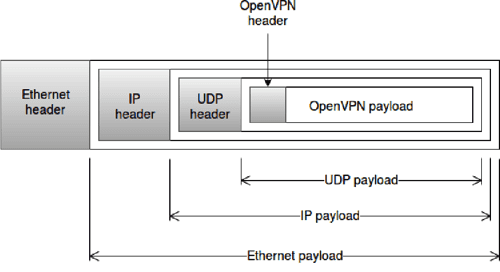
\includegraphics[width=8cm]{figure/OVPN_packet.png}
    \caption{Dettaglio di un pacchetto OpenVPN}
\end{figure}

La struttura mostrata si applica a tutti i pacchetti OpenVPN; tuttavia, differenti pacchetti avranno differenti payloads.


\noindent \textbf{Secure Socket Layer/Transport Layer Security VPNs}
Il protocollo Transport Layer Security, originariamente noto come Secure Socket Layer, è un protocollo progettato per garantire una connessione sicura attraverso una rete non sicura. TLS permette autenticazione di client e server, integrità dei dati e confidenzialità. Per l'autenticazione usa i certificati X.509 \cite[RFC5280]{RFC5280} con una crittografia asimmetrica e si occupa di negoziare una chiave di sessione simmetrica.
Un vantaggio delle VPN SSL rispetto a quelle basate su IPSec è che riescono a lavorare anche in reti protette da firewall molto stringenti, in quanto la maggior parte delle aziende non filtra il traffico TCP sulla porta 443, essendo normalmente usato dai dipendenti per accedere a Internet. OpenVPN di default utilizza la porta 1194 UDP, ma, nel caso quella porta fosse chiusa, può utilizzare la 443 TCP.


\subsubsection{Tunnel TCP vs UDP}
Premesso che attraverso i tunnel VPN passa traffico sia TCP che UDP, anche i tunnel stessi possono essere realizzati con connessioni TCP o UDP.

Il protocollo TCP utilizza notevoli algoritmi per assicurare un recapito corretto dei dati al destinatario. Avere due connessioni TCP una dentro l'altra forzerà gli algoritmi di entrambe le connessioni a lavorare in parallelo. Non essendo TCP progettato per lavorare in quella condizione, si potrebbe andare incontro a problemi quali il \emph{retransmission problem}, \emph{TCP meltdown} e doppia ritrasmissione. Questi problemi potrebbero verificarsi nel momento in cui entrambe le connessioni stanno tentando di ritrasmettere pacchetti.

Tutto ciò non vale per il protocollo UDP, che come descritto precedentemente, è un protocollo non connesso senza nessuna garanzia che il messaggio raggiunga correttamente il destinatario. A discapito dell'affidabilità, si possono ottenere velocità di trasmissione notevolmente superiori.

TCP potrebbe rivelarsi la scelta migliore solo nel caso in cui si debba creare un tunnel che passi attraverso una rete instabile, o attraverso una rete che applica forti censure.

\subsubsection{Cifratura}
OpenVPN utilizza un protocollo di sicurezza personalizzato e SSL/TLS per lo scambio delle chiavi. Usa OpenSSL per la cifratura, dunque è disponibile un ampio numero di algoritmi di cifratura, in particolare basati su AES \cite[RFC3826]{RFC3826}. Quello di default è AES-256-GCM, che garantisce un ottimo livello di sicurezza, specialmente riguardo confidenzialità, autenticazione dell'origine e integrità dei dati.
OpenVPN supporta la Perfect Forward Secrecy, un meccanismo che garantisce che le chiavi di cifratura vengano cambiate automaticamente ad intervalli regolari. Dunque, se anche una chiave venisse compromessa, soltanto una piccola porzione di dati verrebbe esposta.

\subsubsection{Autenticazione}
A differenza della modalità Preshared Static Key, la modalità TLS (preferita) usa il protocollo TLS per autenticare, instaurare una connessione sicura ed effettuare lo scambio delle chiavi simmetriche di sessione tra i peers. L'uso di TLS non solo offre un metodo automatico e sicuro per la distribuzione delle chiavi simmetriche, ma anche un modo per rinnovare tali chiavi in qualsiasi momento della comunicazione.
Questo aspetto della modalità TLS offre ciò che è chiamato Perfect Forward Secrecy, che non è presente nella modalità PSK.
I due step principali del protocollo TLS, a grandi linee, sono:

\begin{enumerate}
    \item negoziazione della connessione TLS: entrambi i lati della connessione si autenticano scambiandosi i certificati e verificando i certificati del lato opposto; se l'autenticazione ha successo, il protocollo procede allo step due; altrimenti, la connessione viene terminata;
    \item le chiavi di sessione sono negoziate attraverso il canale TLS sicuro appena stabilito.
\end{enumerate}


\subsubsection{Misure di sicurezza aggiuntive}
OpenVPN offre diverse funzionalità di sicurezza: cifratura fino a 256-bit attraverso la libreria OpenSSL, anziché supportare IKE; lavora in user space, senza quindi necessità di effettuare operazioni sullo stack IP, e quindi operazioni kernel; ha la possibilià di far cadere i privilegi di root; entrare in una \emph{chroot jail} dopo l'inizializzazione; applicare un SELinux context dopo l'inizializzazione; offre supporto alle smartcard attraverso i token basati su PKCS 11.

\subsubsection{Considerazioni}
Si tratta di una soluzione per VPN matura e flessibile, con supporto a meccanismi di sicurezza all'altezza delle richieste.
Essendo una VPN che lavora al livello $7$ del modello OSI, fa un uso intensivo della CPU. Questo, tuttavia, al giorno d'oggi non è più un grave problema, visto che di potenza computazionale se ne può avere in abbondanza con costi moderati.
Un fattore invece più penalizzante è l'overhead generato dal fatto che si tratta di un software che esegue in user-space, richiedendo dunque molteplici copie dei dati tra kernel-space e user-space.
OpenVPN è più semplice da installare e configurare rispetto a IPSec; tuttavia, le personalizzazioni possibili sono moltissime, che mantengono considerevole il rischio di errori di configurazione.

%--------------------------------------------------------------------------------------------------------------------------------------------Wireguard
\subsection{WireGuard}
WireGuard è una soluzione VPN open-source, che fa della semplicità di configurazione e delle prestazioni i suoi pilastri fondamentali.
\subsubsection{Panoramica}
In IPSec, si ha una separazione netta tra il livello che si occupa dello scambio dati (IKE) e il livello di trasformazione (AH/ESP). Seppure sia una saggia separazione del punto di vista semantico, e decisamente corretta da un punto di vista di rete, ha lo svantaggio di aumentare la complessità implementativa.
WireGuard, anziché implementare questa separazione, crea un'interfaccia di rete virtuale che può essere amministrata con le utility standard \texttt{ip} e \texttt{ifconfig}. Dopo aver configurato questa interfaccia con una chiave privata (e opzionalmente una PSK) e le varie chiavi pubbliche dei peers con cui dovrà comunicare in maniera sicura, la connessione è pronta ad essere instaurata. Scambio di chiavi, connessioni, disconnessioni e via dicendo avvengono dietro le quinte, e l'amministratore non deve configurare nessuno di questi aspetti.
Le regole di firewalling possono essere configurate usando i tool standard, con la garanzia che i pacchetti che provengono da un'interfaccia di WireGuard saranno autenticati e cifrati. Per la sua semplicità, WireGuard è apparentemente meno incline a errori di configurazione rispetto a IPSec.

WireGuard è in grado di instaurare esclusivamente tunnel di livello 3. Con questo approccio è infatti più semplice assicurare autenticità e origine dei pacchetti. Supporta sia IPv4 che IPv6 e può incapsulare sia v4-in-v6 che v6-in-v4.

WireGuard si concentra sulla semplicità e su una codebase facilmente ispezionabile, essendo allo stesso tempo estremamente performante e adatto a diversi ambienti. Combinando lo scambio di chiavi e la cifratura a livello 3 in un unico meccanismo e utilizzando un'interfaccia di rete virtuale anziché un livello di trasformazione, WireGuard rompe con la tradizione per perseguire una soluzione  solida dal punto di vista progettuale, apparentemente più pratica e sicura.

A partire dalla versione 5.6 del kernel Linux, WireGuard verrà incluso nel kernel stesso.
\subsubsection{Protocolli utilizzati}
Nell'implementazione di WireGuard, sono utilizzati i seguenti protocolli:
\begin{itemize}
    \item \textbf{ChaCha20} per la cifratura simmetrica, autenticata con Poly1305, utilizzando AEAD, come specificato in \cite[RFC7539]{RFC7539}
    \item \textbf{Curve25519} come Elliptic-curve Diffie-Hellman, un protocollo per la negoziazione delle chiavi
    \item \textbf{BLAKE2s} per hashing e hashing con chiave, descritto in \cite[RFC7693]{RFC7693}
    \item \textbf{SipHash24} come chiavi per hashtables
    \item \textbf{HKDF} come funzione per la derivazione delle chiavi, descritto in \cite[RFC5869]{RFC5869}
\end{itemize}

\subsubsection{Cifratura}
Dal punto di vista della cifratura utilizzata da WireGuard, rompe la tradizione delle altre soluzioni. Infatti, è intenzionalmente privo di flessibilità per quel che riguarda la scelta dei cifratori e dei protocolli utilizzati. Se vengono trovate falle in quelli scelti in fase di progettazione, tutti i terminali avranno bisogno di essere aggiornati. Come dimostrato dalla continua scoperta di vulnerabilità all'interno del protocollo TLS, dare la possibilità di scegliere quale cifrario usare aumenta enormemente la complessità.

\subsubsection{Autenticazione}
Per la distribuzione delle chiavi, WireGuard si ispira a OpenSSH, dove i due peers si scambiano le proprie chiavi pubbliche statiche. Il meccanismo con cui lo scambio avviene è basato sull'handshake \texttt{Noise IK} di Noise \cite{Noise}. Dopo lo scambio delle chiavi, il peer che non ha iniziato la connessione deve aspettare ad usare la sessione fino a che non riceve un pacchetto cifrato dall'iniziatore, che dà conferma delle chiavi.
Le chiavi pubbliche sono lunghe 32 bytes e possono essere facilmente rappresentate con una codifica Base64 in 44 caratteri, che semplifica il trasferimento di esse attraverso vari mezzi. È supportata anche la Perfect Forward Secrecy, illustrata precedentemente.

\subsubsection{Considerazioni}
La semplicità di installazione è sicuramente un fattore che in ambienti piccoli ha la sua rilevanza; insieme alle prestazioni elevate, la rendono una soluzione da valutare al momento di installare un servizio VPN.
Le possibilità di configurazione sono estremamente minimali. Commettere un errore in fase di configurazione diventa così estremamente meno probabile, a discapito della possibilità di personalizzazione.
Tuttavia, si può comunque contare su scelte di progettazione all'avanguardia e in grado di soddisfare, quantomeno al momento della scrittura della tesi, i più elevati requisiti di cifratura.
Inoltre, l'integrazione di WireGuard all'interno del kernel Linux è simbolo del fatto che si tratta ormai di una soluzione matura e navigata.